
\documentclass[12pt,letterpaper]{article}

\usepackage[T1]{fontenc}
\usepackage{ae,aecompl}
\usepackage[utf8]{inputenc}
\usepackage{lmodern}
\usepackage{tikz}
\usetikzlibrary{shapes.multipart}

\begin{document}

  \begin{center}
    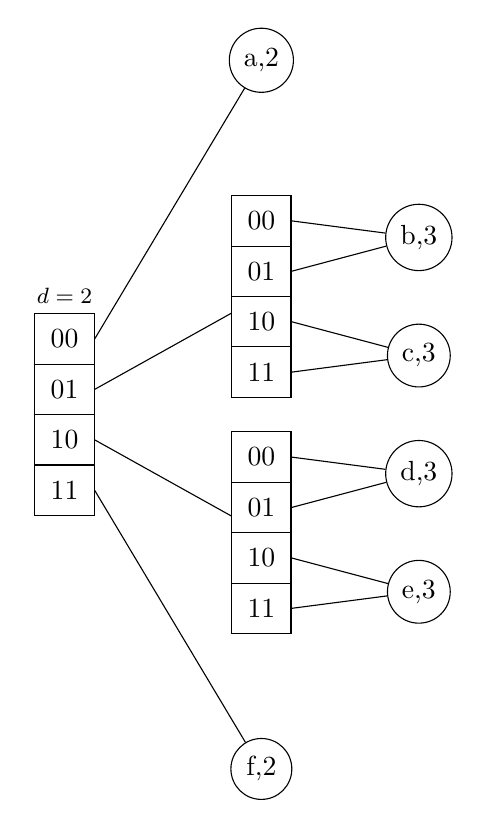
\begin{tikzpicture}[
      grow=right,
      level 1/.style={sibling distance=3cm,level distance=2.5cm},
      level 2/.style={sibling distance=1.5cm,level distance=2cm},
     % edge from parent/.style={draw=none},
      pointer/.style={thick, shorten >=5pt, ->,draw},
      dpointer/.style={draw},
      edge from parent/.style={draw=none},
      every label/.style={font=\footnotesize,draw=none},
      tree/.style={rectangle ,draw, text ragged, inner sep=2mm,minimum width=5mm},
      leaf/.style={circle, draw, inner sep=1mm,minimum width=5mm}
      ]


      \node[tree,label={$d=2$},rectangle split, rectangle split parts=4] (directory) {
        \nodepart{one} 00
        \nodepart{two} 01
        \nodepart{three} 10
        \nodepart{four} 11
      }
        child {
            node[leaf] (firstnode) {f,2}
        }
        child {
            node [tree, rectangle split, rectangle split parts=4](firsttree){
                \nodepart{one} 00
                \nodepart{two} 01
                \nodepart{three} 10
                \nodepart{four} 11
            }child{
                node[leaf] (firstfirstnode) {e,3}
            }
            child{
                node[leaf] (firstsecondnode) {d,3}
            };
        }
        child {
            node [tree, rectangle split, rectangle split parts=4](secondtree){
                \nodepart{one} 00
                \nodepart{two} 01
                \nodepart{three} 10
                \nodepart{four} 11
            }child{
                node[leaf] (secondfirstnode) {c,3}
            }
            child{
                node[leaf] (secondsecondnode) {b,3}
            };
        }
        child {
            node[leaf](lastnode) {a,2}
        };

      %level one edges
      \path(directory.four east) edge (firstnode);
      \path(directory.three east) edge (firsttree);
      \path(directory.two east) edge (secondtree);
      \path(directory.one east) edge (lastnode);
      
      %level two edges
      \path(firsttree.four east) edge (firstfirstnode);
      \path(firsttree.three east) edge (firstfirstnode);
      \path(firsttree.two east) edge (firstsecondnode);
      \path(firsttree.one east) edge (firstsecondnode);
      
      \path(secondtree.four east) edge (secondfirstnode);
      \path(secondtree.three east) edge (secondfirstnode);
      \path(secondtree.two east) edge (secondsecondnode);
      \path(secondtree.one east) edge (secondsecondnode);
    \end{tikzpicture}
  \end{center}

\end{document}
